76. \begin{figure}[ht!]
\center{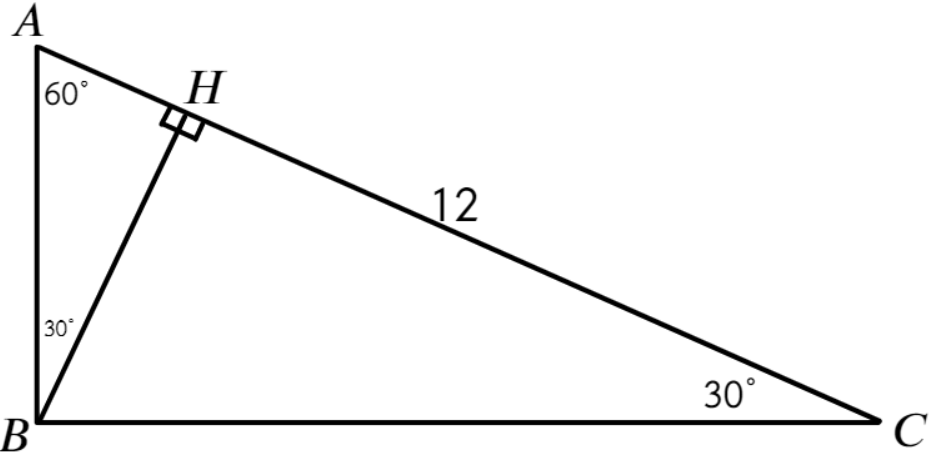
\includegraphics[scale=0.35]{g76.png}}
\end{figure}\\
Пусть $\angle A=60^\circ,$ тогда $\angle C=90^\circ-60^\circ=30^\circ,\ \angle ABH=90^\circ-60^\circ=30^\circ.$ По теореме о катете, лежащем напротив угла в $30^\circ,$ для треугольников $ABH$ и $ABC$ имеем $AB=2AH,\ AC=2AB=4AH,\ HC=4AH-AH=3AH=12,\ AH=4,\ AC=4\cdot4=16.$\\
